The data race detection technique presented in this work performs the analysis after the program has finished execution (post-mortem analysis). To improve the efficiency of analysis at run time, this paper presents a dynamic improvement for structured parallel programs. This technique is called on-the-fly data race detection. 

The data race detection is run on a region as soon as await finishes execution on that region (i.e., \textsc{Await-done} fires). If no race is reported, all the nodes belonging to that region are merged into an equivalent master node that represents the region. The transformation preserves the partial order relative to other tasks. The variables accessed by the tasks in the region are added to the master node. 

To implement this technique, the \textsc{Await-done} rule has been modified as follows. The $\mathrm{join}$ and $\mathrm{meet}$ nodes for set of nodes connected to the current node of task executing \textsc{Await-done} are identified.

\begin{definition}
$\mathrm{Join}:$ In a partially ordered set ($N, \preceq$), an element $n_0$ is a $\mathrm{join}$ of two unordered elements $n_1$ and $n_2$ if the following conditions hold:
\begin{itemize}
\item $n_0 \prec n_1$ and $n_0 \prec n_2$ (i.e., $n_0$ happens before $n_1$ and $n_2$).
\item For any element $n$ in $N$, such that $n \prec n_1$ and $n \prec n_2$, we have $n \prec n_0$.
\end{itemize}
\end{definition}

A $\mathrm{join}$ is the least upper bound for a subset of elements in the partially ordered set. Conversely, a $\mathrm{meet}$ is greatest lower bound for the elements in the partially ordered set. $\mathrm{Join}$ and $\mathrm{meet}$ are symmetric duals with respect to order inversion. 

\begin{definition}
$\mathrm{Meet}:$ In a partially ordered set ($N, \preceq$), an element $n_0$ is a $\mathrm{meet}$ of two unordered elements $n_1$ and $n_2$ if the following conditions hold:
\begin{itemize}
\item $n_1 \prec n_0$ and $n_2 \prec n_0$ (i.e., $n_0$ happens after $n_1$ and $n_2$).
\item For any element $n$ in $N$, such that $n_1 \prec n$ and $n_2 \prec n$, we have $n_0 \prec n$.
\end{itemize}
\end{definition}

\begin{definition}
A $\mathrm{lattice}$ is defined as a partially ordered set such that every pair of elements has a unique $\mathrm{join}$ and a unique $\mathrm{meet}$.
\end{definition}

\begin{lemma}
A computation graph of a structured parallel program is a $\mathrm{lattice}$.
\end{lemma}
\begin{proof}
Structured parallel programs have a restriction of joining all unsynchronized tasks to the main task at the end of program execution. The node that represents the main task when the program starts execution acts as $\mathrm{join}$ node for all the nodes in the graph and the last await node acts as $\mathrm{meet}$ node. For any pair of nodes $n_1$ and $n_2$, either the nodes are ordered or unordered. If the nodes are ordered, $n_1 \prec n_2$ or vice versa, then there is a unique $\mathrm{meet}$ or $\mathrm{join}$ depending on the ordering. For example, if $n_1 \prec n_2$, then $n_1$ is the $\mathrm{join}$ and $n_2$ is the $\mathrm{meet}$.  

If, however, the nodes are unordered, then it needs to be proven that the $\mathrm{meet}$ and $\mathrm{join}$ are unique based on the structure of the graph. Consider the rules that add nodes to the graph. Nodes are added when \textsc{Post}, \textsc{Await-next} or \textsc{Ewait} rule fires. A \textsc{Post} rule is fired when a new task is created. The parent task creates branching in the graph by adding nodes to represent the parent and child task that executes in parallel. Since every task can only have a single parent, the $\mathrm{join}$ node for the unordered nodes is unique. Tasks synchronize only on completion when \textsc{Await-next} or \textsc{Ewait} rule fires. Since structured parallel programs do not allow task passing, tasks are bound to join to their parent/ancestor task only. Therefore, they cannot be cross-edges in the computation graph. Hence, a pair of unordered nodes can have only a unique $\mathrm{meet}$. Therefore, a computation graph of a structured parallel program is a $\mathrm{lattice}$.
\end{proof}

\begin{figure}
  \begin{center}
    \mprset{flushleft}
    \begin{mathpar}
    \inferrule[Await-done]
		{
		  m(r) = \emptyset \\                  
		  G^\prime = \mathrm{subGraph}(\forall n^\prime, \tuple{n^\prime, n} \in E) \\
		  DRF(G^\prime) = true \\
		   n_1 = \mathrm{fresh()} \\                 
		  N = N \setminus N^\prime \cup \{n_1\} \\
		  E = E \setminus E^\prime \\
		 \delta(n_1) = \bigcup_{n^\prime \in N^\prime} \delta(n^\prime) \\
		 \omega(n_1) = \bigcup_{n^\prime \in N^\prime} \omega(n^\prime)
		}
		{
		  C[\tuple{\ell, S[\textbf{await}~r],\vec{r_\delta},\vec{r_\omega},d, n}, m] \rightarrow 
		  C[\tuple{\ell, S[\textbf{skip}],\vec{r_\delta},\vec{r_\omega},d, n_1}, m]
		}
    \end{mathpar}
  \end{center}
  \caption{\textsc{Await-done} rule updated for on-the-fly data race detection.}
  \label{fig:sem:otf}
\end{figure}

The modified \textsc{Await-done} rule for on-the-fly data race detection is presented in \figref{fig:sem:otf}. $\mathrm{subGraph}$ takes a set of nodes, finds the meet/join, and then extracts everything, inclusive, as a sub-graph. The sub-graph for the set of nodes connected to $n$ is extracted using $\mathrm{subGraph}$. This sub-graph is verified using Algorithm \ref{algo:drd}. If this sub-graph is data race free, the nodes in this sub-graph are deleted from the computation graph. A new master node $n_1$ is added to the graph in place of this sub-graph. The region variables accessed by the nodes in the sub-graph are added to $n_1$.

\begin{figure}
  \begin{center}
    \begin{lstlisting}[mathescape=true]
  proc main(var n : int)
  	n := 1;
  	post $r_1 \leftarrow p_1~n~\varepsilon~\{r_1\}~\{r_1\}~\lambda v. n := n + v$;
	await $r_1$
 proc $p_1$(var n : int)
 	post $r_2 \leftarrow p_2~n~\varepsilon~\{r_1\}~\{r_1\}~\lambda v. n := n + v$;
  	post $r_2 \leftarrow p_3~n~\varepsilon~\{r_1\}~\{r_1\}~\lambda v. n := n + v$;  	  	
	await $r_2$
 proc $p_2$(var n : int)
	$\texttt{l}(r_2) := n$ 
 proc $p_3$(var n : int)
	$\texttt{l}(r_2) := n$
\end{lstlisting}
  \end{center}
  \caption{A parallel program with nested regions.}
  \label{fig:nested-regions}
\end{figure}

\begin{figure}
\centering
  \subfigure[Comp graph for parallel program with nested regions]{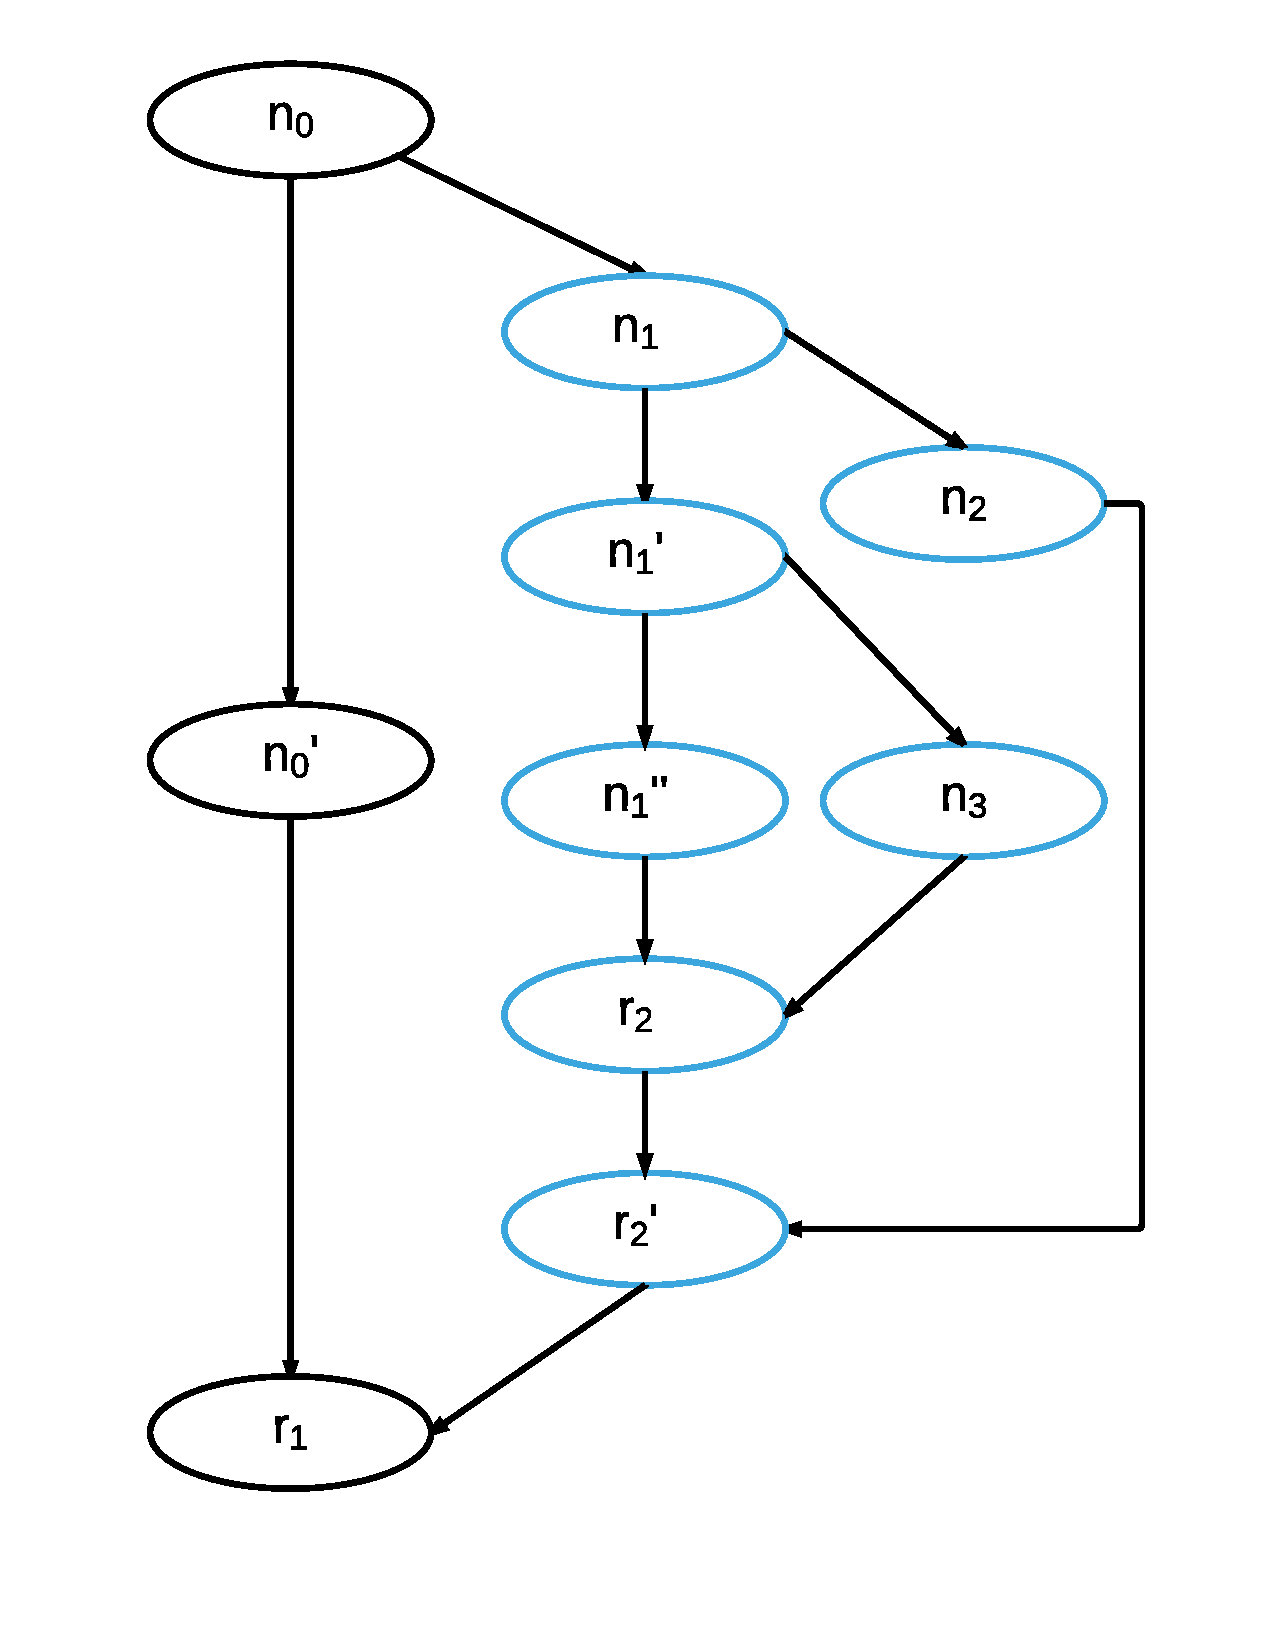
\includegraphics[scale=0.375]{../figs/Fig7-a.pdf}}
  \subfigure[Comp graph with master node]{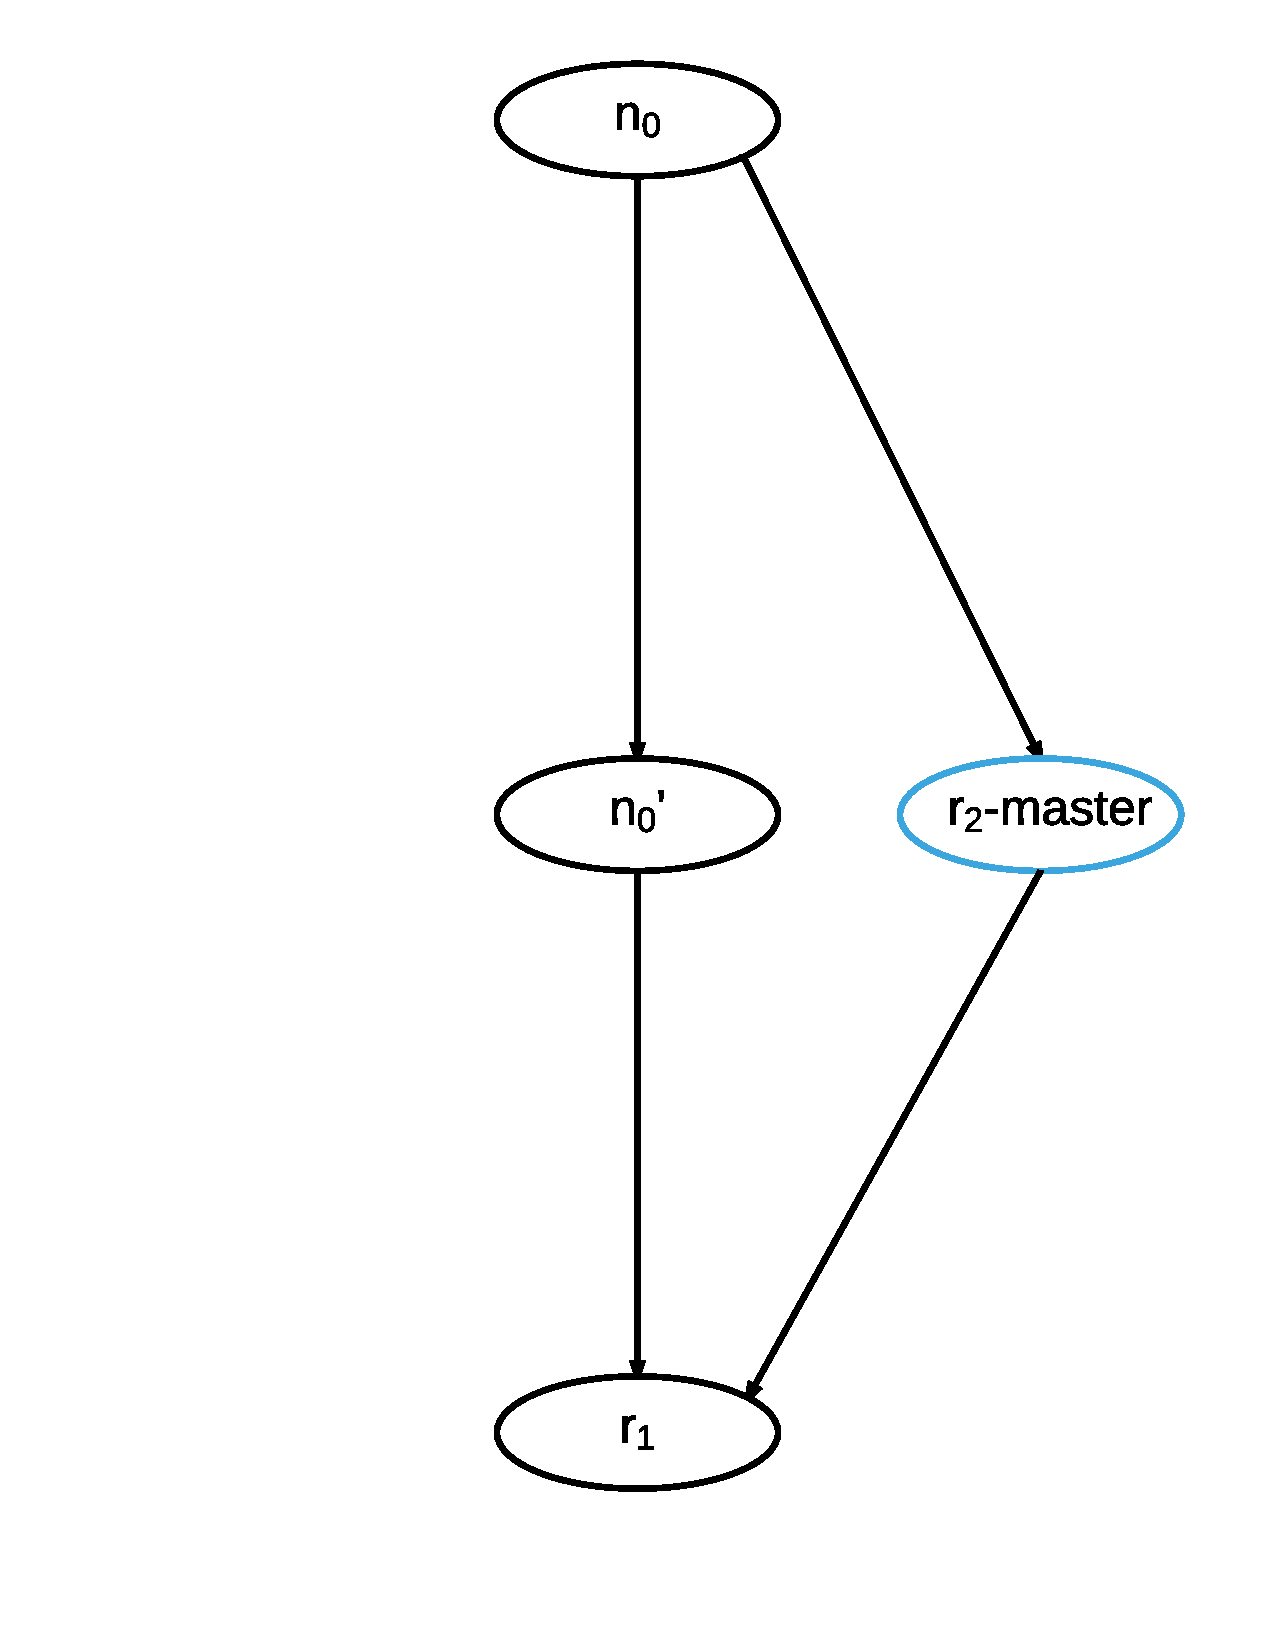
\includegraphics[scale=0.375]{../figs/Fig7-b.pdf}}
  \caption{Computation graph of example in \figref{fig:nested-regions}.}
   \label{fig:cg-nested-regions}
\end{figure}

\figref{fig:nested-regions} shows an example of a parallel program with nested regions. The $main$ task spawns a task $t_1$ in region $r_1$. Task $t_1$ spawns two new tasks $t_2$ and $t_3$ in region $r_2$. The await on $r_2$ is executed before await on $r_1$ making the regions nested. All the tasks have read/write access to region variable $r_1$. As soon as the await on region $r_2$ finishes execution, on-the-fly analysis is run on this region to check for data races in the nodes belonging to this region. If a race is not reported, a master node is added to the graph that represents region $r_2$ and the program is executed further. The computation graph for this example is shown in \figref{fig:cg-nested-regions}(a). The nodes that are used to find the $\mathrm{meet}$ and $\mathrm{join}$ are $r_2$ and $n_2$. The nodes highlighted in blue denote the sub-graph that is replaced by a master node if the region is data race free. \figref{fig:cg-nested-regions}(b) shows the computation graph with a master node inserted in place of region $r_2$.
